%!TEX root = ../../Main.tex
\graphicspath{{Chapters/Struktur/}}
%-------------------------------------------------------------------------------

\section{Graphic display driver}

Som brugergrænseflade i dette projekt bruges et ITDB02, som er valgt da der tidligere er arbejdet med netop dette produkt. Dertil kommer ILI9341 som driver til selve display'et. 

Driver softwaren til hele displayet, er delt op i flere forskellige cpp filer, dette er gjort for at gøre koden mere overskuelig, og gøre funktionaliteten mere effektiv. Herunder forsøges at gøre et overblik over de forskellige cpp filer og deres integeren. 


\begin{figure}[H]
	\centering
	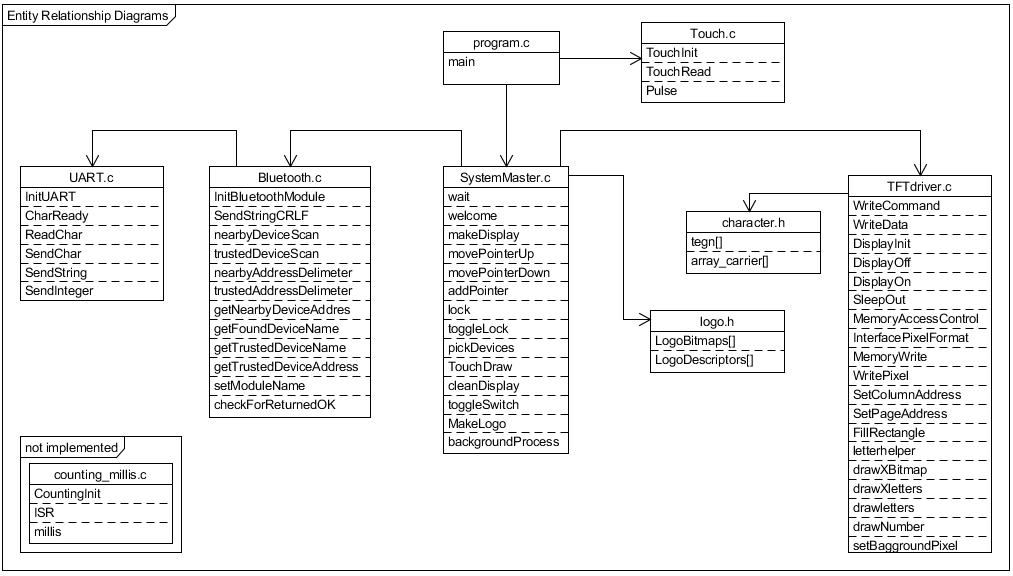
\includegraphics[width = 300 pt]{Img/Entity.png}
	\caption{Entity Relationship Diagrams}
	\label{fig:Konceptbillede}
\end{figure}
 
---Skriv noget når det hele er færdig her



